\documentclass[french]{article}
\usepackage[utf8]{inputenc}
\usepackage[T1]{fontenc}
\usepackage{lmodern}
\usepackage[a4paper]{geometry}
\usepackage{babel}
\usepackage{graphicx}
\usepackage[linkcolor=black,colorlinks=true,linkbordercolor={0 0 0},urlbordercolor={0 0 0},urlcolor=black]{hyperref}
\usepackage{listings}
\lstdefinestyle{customstyle}{
	basicstyle=\footnotesize,
	breakatwhitespace=false,         
	breaklines=true,                 
	captionpos=b,                    
	keepspaces=true,
	showspaces=false,
	showstringspaces=false,
	showtabs=false,
	tabsize=4,
	frame=single, %lines
}
\lstset{style=customstyle}
\title{Compilateur FreeBasic vers C\\\large{Rapport de projet}}
\author{Anthony Pena}
\date{10 Avril 2015}

\begin{document}

\maketitle{}
\tableofcontents{}
\newpage{}
\part{Introduction}

Dans le cadre du cours de Compilation, il nous a été demandé de réaliser un petit compilateur. Le compilateur a pour objectif de compiler du code écrit en FreeBasic vers du code en langage C.

Pour rappel un compilateur fonctionne en deux étapes. La première est appelé analyse lexicale (réalisé ici avec OCamlLex), elle permet de définir les éléments faisant partie d'un langage. La seconde est une étape d'analyse sémantique (réalisé ici avec OCamlYacc) qui permet de vérifier que les différents éléments du langage sont bien ordonnés et donc crée du sens.

L'ensemble des codes sources et les éléments nécessaires à la compilation sont disponible à l'adresse suivante : \url{https://github.com/kuroidoruido/ColorBASIC}.

\part{Éléments généraux}
% sous-ensemble restreint voulu => montrer un peu d'intérêt
% exemple d'éléments concrètement reconnu dans les tests
Pour commencer il est important de préciser que le compilateur rendu n'est pas en mesure de compiler l'ensemble du langage FreeBasic, seulement un sous-ensemble. Le choix a été fait pour couvrir quelques éléments intéressant d'un point de vue compilation et parce que le but final n'étant que pédagogique et pas de vraiment réaliser un compilateur FreeBasic vers C. De plus sans que cela soit détaillé dans chaque section, il est possible de visualiser l'ensemble des types de cas testés pour chaque élément via les fichiers en basic du dossier \emph{test/} du répertoire GitHub.

Il peut être utile aussi préciser que certains choix ont été fait du fait que FreeBasic et C sont différents et possèdes des fonctions de base différentes. Pour combler cela il a été fait le choix de systématiquement inclure les bibliothèques stdlib et stdio en C pour accéder par exemple à la fonction printf. On retrouve aussi l'ajout d'une fonction main qui englobe l'ensemble du code source du programme alors qu'en FreeBasic le fichier principale est déjà l'équivalent de cette fonction.

Il est a noté qu'il a été fait le choix de considérer que le code en FreeBasic est valide et compile déjà via un compilateur standard (tels que \emph{fgc}) et que le code en sorti se devait d'être compilé avec un compilateur C standard tel que \emph{gcc}. Cela implique qu'il y a des vérifications d'effectués mais surtout sur la bonne définition des variables et donc celle-ci est incomplète. Cela implique aussi qu'il n'a pas été apporté de soin à ce que le code en sortie soit convenablement lisible par un humain et donc l'indentation n'est pas effectuée par exemple.

Il est aussi a noté que pour simplifier la lecture du code Yacc et Lex, le choix a été fait de ne pas conserver le caractère non-sensible à case de FreeBasic. En effet FreeBasic considère comme équivalent "PRINT", "Print", "PRint", "PrinT", etc. or cela obligeait a écrire avec une regex permettant une reconnaissance de toutes ces variantes ce qui est fastidieux et peu intéressant. Il a donc été pris comme convention que les instructions ou structures de contrôles FreeBasic seraient écrit en capital (par exemple "IF" ou "PRINT") et que les types de bases seraient écrit avec une lettre majuscules suivit de minuscule (par exemple "String" ou "Integer").

\part{Éléments reconnus}

\section{Variables et affectations}

Le langage FreeBasic reconnaît nativement les entiers, les chaînes de caractères (3 types), les floatants, etc. Pour l'exemple il a été fait le choix de se limiter à 2 types : les entiers (\emph{Integer}) et chaînes de caractères (\emph{String}). Le compilateur reconnaît les déclarations, les affectations simple ainsi que les affectations par expression entière (voir \ref{ssec:expr-entiere}) dans le cas d'une variables numérique.

Il est donc possible de déclarer une variable puis de lui assigner une valeur (le type étant vérifié à ce moment, on ne peut pas affecter une String à un Integer par exemple) ou bien tout faire en une seule ligne.

\section{Commentaires}

En FreeBasic il est possible de définir des commentaires mono-ligne ou multi-lignes. Les commentaires multi-lignes démarre par "~/'~" et se termine par "~'/~". Les commentaires mono-ligne peuvent commencé soit par "~'~" soit "REM".

Dans le cas des commentaires il a été fait le choix de prendre tous les cas en compte. De ce fait peu importe le type de commentaire ou sa position (fin de ligne, ligne complète, multi-ligne, etc.) il sera pris en compte et compilé en commentaire C.

\section{Conditions}

Comme tout langage le FreeBasic permet d'utiliser un certain nombre de structure conditionnel, ici il a été fait le choix de ne conserver que le if avec ou sans elseif et avec ou sans else. Le compilateur reconnaît toutes les variantes de if then elseif else tout en s'assurant qu'on ne validera pas un if suivit de deux else par exemple.

Il est aussi pris en compte la possibilité d'imbriquer des structures de if dans le bloc then ou elseif ou else. De la même façon il est possible d'y mettre une boucle par exemple. La condition du if est exprimé sous la forme d'une expression booléenne (voir \ref{ssec:expr-booleenne}).

\section{Boucles}

De la même façon que pour les conditions, il a été fait le choix de n'implémenter qu'un seul type de boucle, la boucle while, car elle est générique en algorithmie et permet de remplacer n'importe quelle autre boucle.

La boucle while en FreeBasic s'écrit via un "WHILE" suivit d'une condition sous forme d'expression booléenne (voir \ref{ssec:expr-booleenne}) puis après un retour à la ligne d'une liste d'instruction terminé par un "WEND". Sa forme est similaire la forme en C.

\section{Fonctions de bases}

Afin de tester le bon fonctionnement du compilateur il était indispensable de reconnaître quelques fonctions de base et il a été choisi PRINT, LOCATE et SLEEP.

PRINT se traduit par la fonction printf en C, celle-ci est fonctionnelle mais limité à un seul argument. Il aurait été possible d'accepter plusieurs mais programmer la génération des motifs pour la fonction printf aurait été coûteux en temps et ce n'était pas l'objectif du projet. Pour respecter le fonctionnement original du PRINT en FreeBasic, un retour à la ligne est ajouté systématiquement à la fin de chaque printf en C.

LOCATE permet de replacer l'emplacement du curseur. L'intérêt de cette fonction n'est pas importante mais celle-ci est facile à implémenter via un appel système à une fonction bash. L'implémentation de celle-ci de cette façon rend par contre ce code non fonctionnel sur Windows par exemple.

La fonction SLEEP, avec pour équivalent la fonction de même nom en C, permet d'effectuer une pause dans le programme, il s'agit donc de nouveau d'une instruction simple à compiler et donc pratique pour les tests.

\section{Expressions}
\subsection{Expressions entières}
\label{ssec:expr-entiere}
Une expression entière est un calcul qui peut être composé librement d'Integer, d'opérateur +, -, * ou /, ainsi que de sous calcul via parenthèse.

\subsection{Expressions booléennes}
\label{ssec:expr-booleenne}

Une expression booléenne est une suite de sous expression de comparaison qui forme une suite d'élément à valeur booléenne et dont le résultat est booléen aussi. De cette façon, ici il est tenu compte des opérateurs de comparaison classique des entiers (=, <> (en C !=), <, >, <=, >=), pour les chaînes de caractères seul l'égalité est reconnue.

\part{Fonctionnement Général}
\section{Utilisation du compilateur}
À partir d'ici nous allons utiliser le code source FreeBasic d'une petite implémentation de la suite de Fibonacci\footnote{\url{https://fr.wikipedia.org/wiki/Suite_de_Fibonacci}}. Ce programme, présenté dans le Listing \ref{lst:exp-basic}, va afficher les 30 premières itérations (en plus des deux valeurs d'initialisation). La version compilé, via le compilateur développé ici, de ce code est présenté  sans aucune modification dans le Listing \ref{lst:exp-c}.

Comme on peut le voir le code original est bien compilé en code C puis placé dans une fonction main avec les inclusions nécessaires. On remarque aussi l'absence de tabulation dans le contenu du while mais ça n'empêche pas sa lisibilité au vu de la simplicité de l'exemple qui montre tout de même la manipulation des entiers, des chaînes de caractères, du while, du print et des affectations. 

\lstset{language=[Visual]Basic,caption=Exemple de programme en FreeBasic,label=lst:exp-basic}
\lstinputlisting{res/fibonacci.bas}

% équivalent C
\lstset{language=C,caption=Exemple compilé en C,label=lst:exp-c}
\lstinputlisting{res/fibonacci.c}

% exécution
\section{Arbre syntaxique}

Bien qu'aucune structure de donnée n'est été mis en place pour représenter l'arbre syntaxique dans le code OCaml, l'arbre est bien présent dans la manière dont sont lu les instructions FreeBasic. En effet la génération du code se fait via concaténation et l'écriture dans le fichier se fait d'un coup, avec l'intégralité du code source C. On obtient donc un arbre qui se construit via des concaténations de chaîne.

La Figure \ref{fig:ast} montre une représentation sous forme d'arbre du programme exemple Listing \ref{lst:exp-basic}.

\begin{figure}[h]
    \centering
    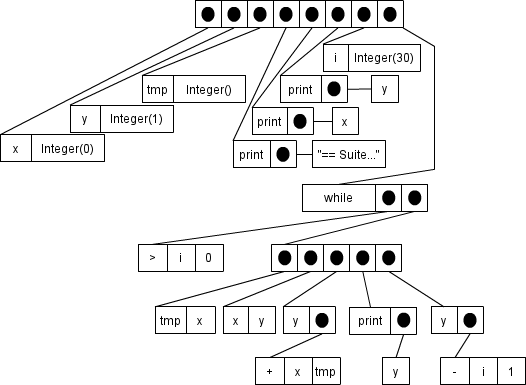
\includegraphics[width=0.9\textwidth]{res/ast.png}
    \caption{Arbre syntaxique équivalent au programme exemple}
    \label{fig:ast}
\end{figure}

\part{Conclusion}

Durant ce projet nous avons pu mettre en pratique les éléments théoriques du cours de Compilateur à travers ce mini compilateur. Cela nous a aussi permis de découvrir l'utilisateur de Lex et Yacc à travers leurs implémentations OCamlLex et OCamlYacc.

\end{document}
